\uuid{LmJU}
\exo7id{7628}
\titre{exo7 7628}
\auteur{mourougane}
\organisation{exo7}
\datecreate{2021-08-10}
\isIndication{false}
\isCorrection{true}
\chapitre{Autre}
\sousChapitre{Autre}

\contenu{
\texte{
Calculer $$\int_{\partial \Delta_2(1)}\frac{z^2+z-1}{z^2(z^2-4)}dz.$$
}
\reponse{
~
 \begin{center} 
 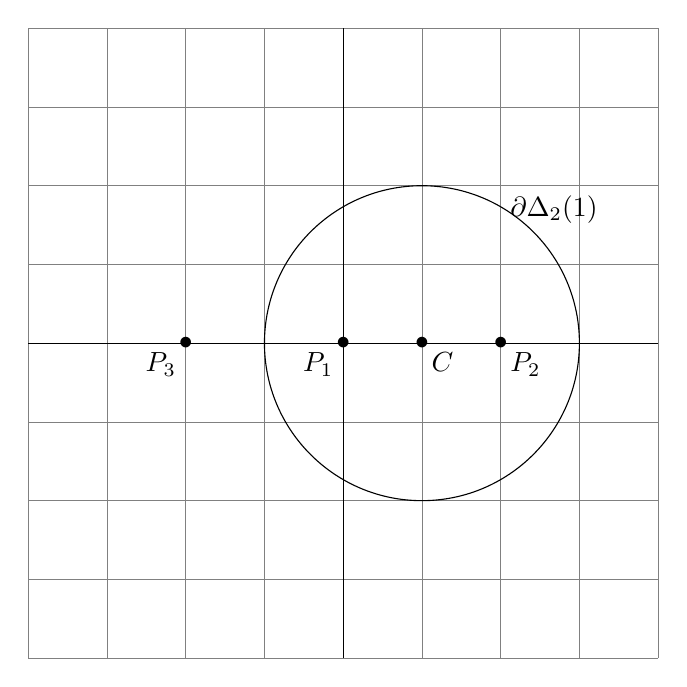
\begin{tikzpicture}
 \draw [step=1cm, gray, very thin](-4,-4) grid (4,4);
 \draw (-4,0) -- (4,0); \draw (0,-4) -- (0,4);
 \draw (0,0) node {$\bullet$}; \draw (0,0) node[below left] {$P_1$};
 \draw (2,0) node {$\bullet$};\draw (2,0) node [below right] {$P_2$};
 \draw (-2,0) node {$\bullet$};\draw (-2,0) node [below left] {$P_3$};
\draw (1,0) node {$\bullet$}; \draw (1,0) node [below right] {$C$} circle (2) ;
\draw (2,2) node[below right] {${\partial \Delta_2(1)}$};
\end{tikzpicture}
\end{center}
On écrit la décomposition en éléments simples de la fraction rationnelle
$$\frac{z^2+z-1}{z^2(z^2-4)}=\frac{5}{16}\frac{1}{z-2}-\frac{1}{16(z+2)}-\frac{1}{4z}+\frac{1}{4z^2}.$$
Les premier et troisième termes correspondent aux pôles simples $P_2$ et $P_1$ à l'intérieur du cercle ${\partial \Delta_2(1)}$.
Donc, 
$$\int_{\partial \Delta_2(1)}\left(\frac{5}{16}\frac{1}{z-2}-\frac{1}{4z}\right)dz=(2i\pi)(\frac{5}{16}-\frac{1}{4})=\frac{i\pi}{8}.$$
Le deuxième terme correspond au pôle $P_3$ à l'extérieur du cercle ${\partial \Delta_2(1)}$ donc, $\int_{\partial \Delta_2(1)}\frac{1}{16(z+2)}dz=0$.
Le dernier terme est l'intégrale sur un chemin fermé de l'application exacte $z\mapsto \frac{1}{4z^2}$ de primitive $z\mapsto -\frac{1}{4z}$.
Donc, $\int_{\partial \Delta_2(1)}\frac{1}{4z^2}dz=0$.
En conclusion, 
$$\int_{\partial \Delta_2(1)}\frac{z^2+z-1}{z(z^2-4)}dz=\frac{i\pi}{8}.$$

Une autre démarche serait : 
on écrit la décomposition en éléments simples de la fraction rationelle
$$\frac{1}{z^2(z^2-4)}=\frac{1}{16}\frac{1}{z-2}-\frac{1}{16(z+2)}-\frac{1}{4z^2}.$$
et donc avec $f(z)=z^2+z-1$ holomorphe sur $\Cc$
$$\frac{z^2+z-1}{z^2(z^2-4)}=\frac{1}{16}\frac{f(z)}{z-2}-\frac{f(z)}{16(z+2)}-\frac{f(z)}{4z^2}.$$
Par le théorème de Cauchy sur les disques, puisque $0$ et $2$ sont dans $\Delta_2(1)$ mais pas $-2$,
\begin{eqnarray*}\int_{\partial \Delta_2(1)}\frac{z^2+z-1}{z^2(z^2-4)}&=&\frac{1}{16}\int_{\partial \Delta_2(1)}\frac{f(z)}{z-2}-\int_{\partial \Delta_2(1)}\frac{f(z)}{16(z+2)}-\int_{\partial \Delta_2(1)}\frac{f(z)}{4z^2}\\
&=&\frac{2i\pi f(2)}{16}-0-\frac{2i\pi f'(0)}{4}=\frac{5i\pi}{8}-\frac{i\pi}{2}
 =\frac{i\pi}{8}.
\end{eqnarray*}
}
}
